\documentclass[a4paper]{article}    % define document layout
%\documentclass[draft]{article}     % use draft option in packages
%-----------------------------
% preamble
%-----------------------------
\usepackage[sumlimits,]{amsmath}    % math equations and formulas
\usepackage[utf8]{inputenc}         % use UTF-8 encoding
\usepackage[english]{babel}         % use English language
\usepackage{graphicx}              % insert images
%\usepackage[draft]{graphicx}        % do not render figures
\usepackage{subcaption}             % multiple images in one figure
\usepackage{hyperref}               % hyperlinks
\usepackage{float}                  % floating objects (figures, tables)
\usepackage{geometry}               % page size and margins
\geometry{a4paper, margin=1in}      % margins
\usepackage{ragged2e}               % text alignment
\usepackage[table]{xcolor}          % change cell color in tables
%\usepackage{multirow}               % merge rows in table
%\usepackage[thinc]{esdiff}          % macros for derivatives

% MATLAB code
\usepackage{listings}
\usepackage{color} %red, green, blue, yellow, cyan, magenta, black, white
\usepackage{xcolor}

\graphicspath{                      % path for figures
    {../figures/} 
    {../figures/Q1/} 
}

\definecolor{codegreen}{rgb}{0,0.6,0}
\definecolor{codegray}{rgb}{0.5,0.5,0.5}
\definecolor{codepurple}{rgb}{0.58,0,0.82}
\definecolor{backcolour}{rgb}{0.95,0.95,0.92}

\lstdefinestyle{mystyle}{
    backgroundcolor=\color{backcolour},   
    commentstyle=\color{codegreen},
    keywordstyle=\color{magenta},
    numberstyle=\tiny\color{codegray},
    stringstyle=\color{codepurple},
    basicstyle=\ttfamily\footnotesize,
    breakatwhitespace=false,         
    breaklines=true,                 
    captionpos=b,                    
    keepspaces=true,                 
    numbers=left,                    
    numbersep=5pt,                  
    showspaces=false,                
    showstringspaces=false,
    showtabs=false,                  
    tabsize=2
}
\lstset{style=mystyle}

%-----------------------------
% body
%-----------------------------
\begin{document}

\begin{figure}
    \centering
    % UNICAMP logo
    \begin{subfigure}{0.45\textwidth}
        \centering
        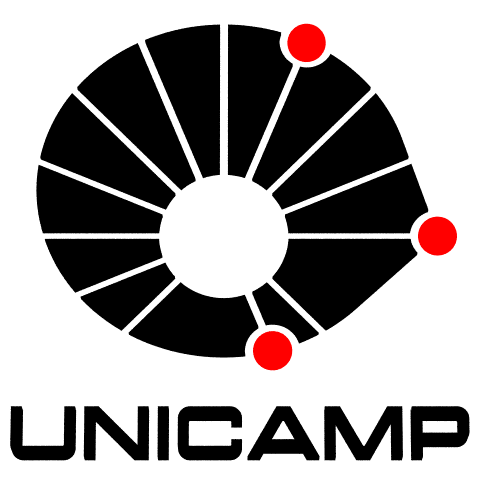
\includegraphics[width=1.5cm]{unicamp}
%        \label{fig:unicamp}
    \end{subfigure}
    \hfill
    % FEEC logo
    \begin{subfigure}{0.45\textwidth}
        \centering
        
\includegraphics[width=1.5cm]{feec}
%        \label{fig:feec}
    \end{subfigure}
\end{figure}

\title{
    \vspace{5cm}
    IA353A - Neural Networks\\
    EC1
    \vspace{1cm}
}
\author{
    Rafael Claro Ito\\
    (R.A.: 118430)
    \vspace{11cm}
}
%R.A.: 118430
%ito.rafael@gmail.com
\date{May 2020}
\maketitle
\newpage

%=================================================
\section*{Question 1}
%=================================================

\addtocounter{section}{1}
%========================
\subsection{SGD}
%========================

%------------------------
\subsubsection{Underdetermined}
%------------------------

% code
\lstinputlisting[language=Octave]{../Q1/sgd_under.m}

% insert plots
\begin{figure}[H]
    \centering
    % digit 0
    \begin{subfigure}{0.48\textwidth}
        \centering
        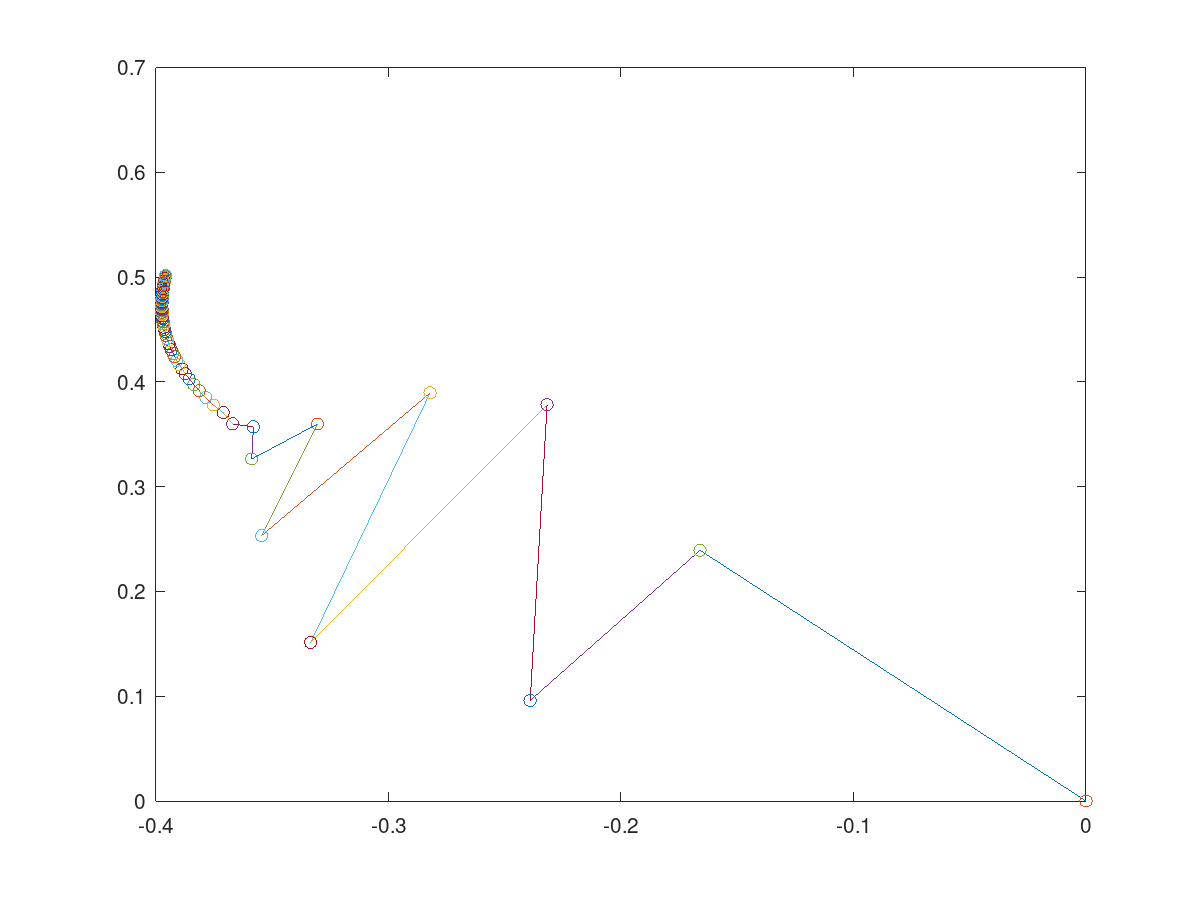
\includegraphics[width=7.5cm]{sgd_under_step_0_1}
        \caption{Progression of W using step of 0.1}
        \label{fig:sgd-under-0_1}
    \end{subfigure}
    \hfill
    % digit 1
    \begin{subfigure}{0.48\textwidth}
        \centering
        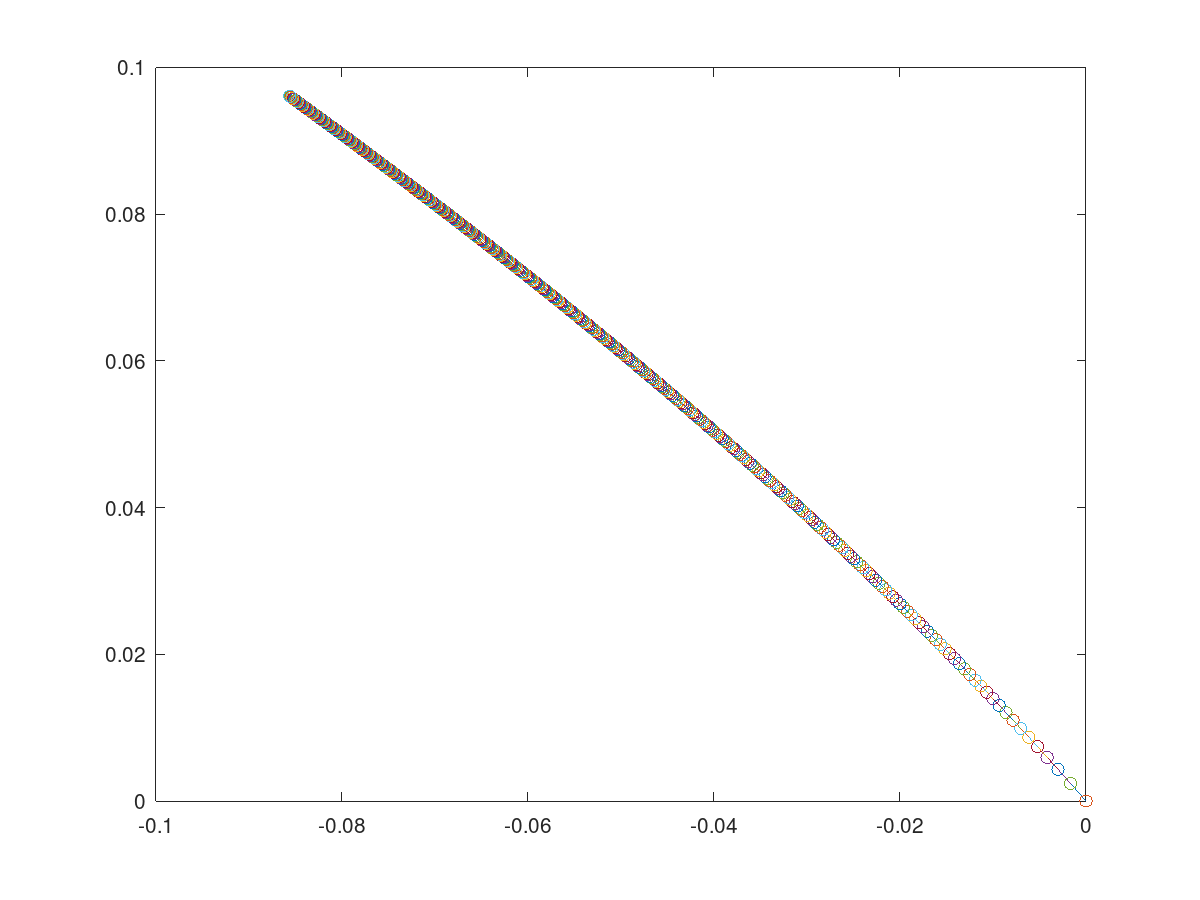
\includegraphics[width=7.5cm]{sgd_under_step_0_001}
        \caption{Progression of W using step of 0.001}
        \label{fig:sgd-under-0_001}
    \end{subfigure}
    \hfill
    % caption and label
    \caption{Progression of W for underdetermined system using SGD}
    \label{fig:sdg-under}
\end{figure}

\newpage

%------------------------
\subsubsection{Overdetermined}
%------------------------

% code
\lstinputlisting[language=Octave]{../Q1/sgd_over.m}

% insert plots
\begin{figure}[H]
    \centering
    % digit 0
    \begin{subfigure}{0.48\textwidth}
        \centering
        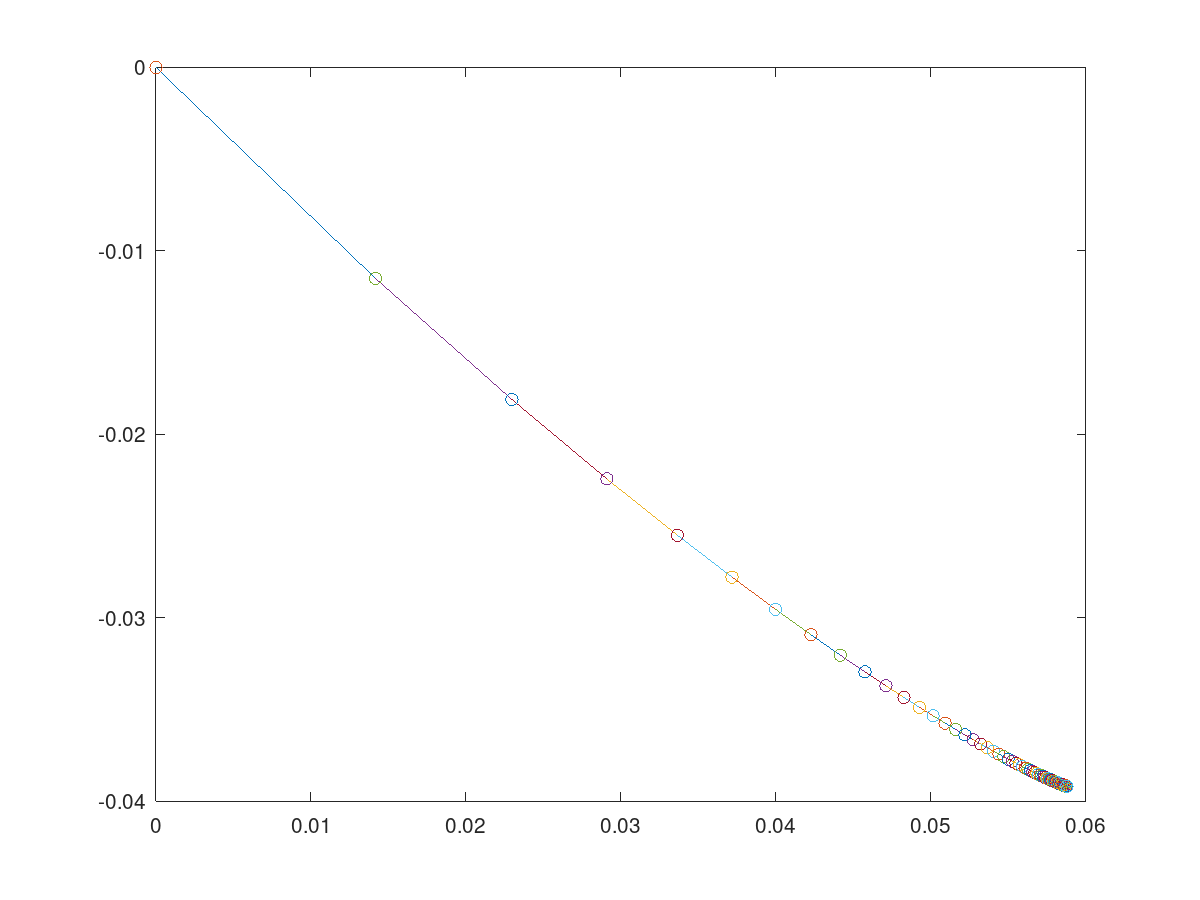
\includegraphics[width=7.5cm]{sgd_over_step_0_1}
        \caption{Progression of W using step of 0.1}
        \label{fig:sgd-over-0_1}
    \end{subfigure}
    \hfill
    % digit 1
    \begin{subfigure}{0.48\textwidth}
        \centering
        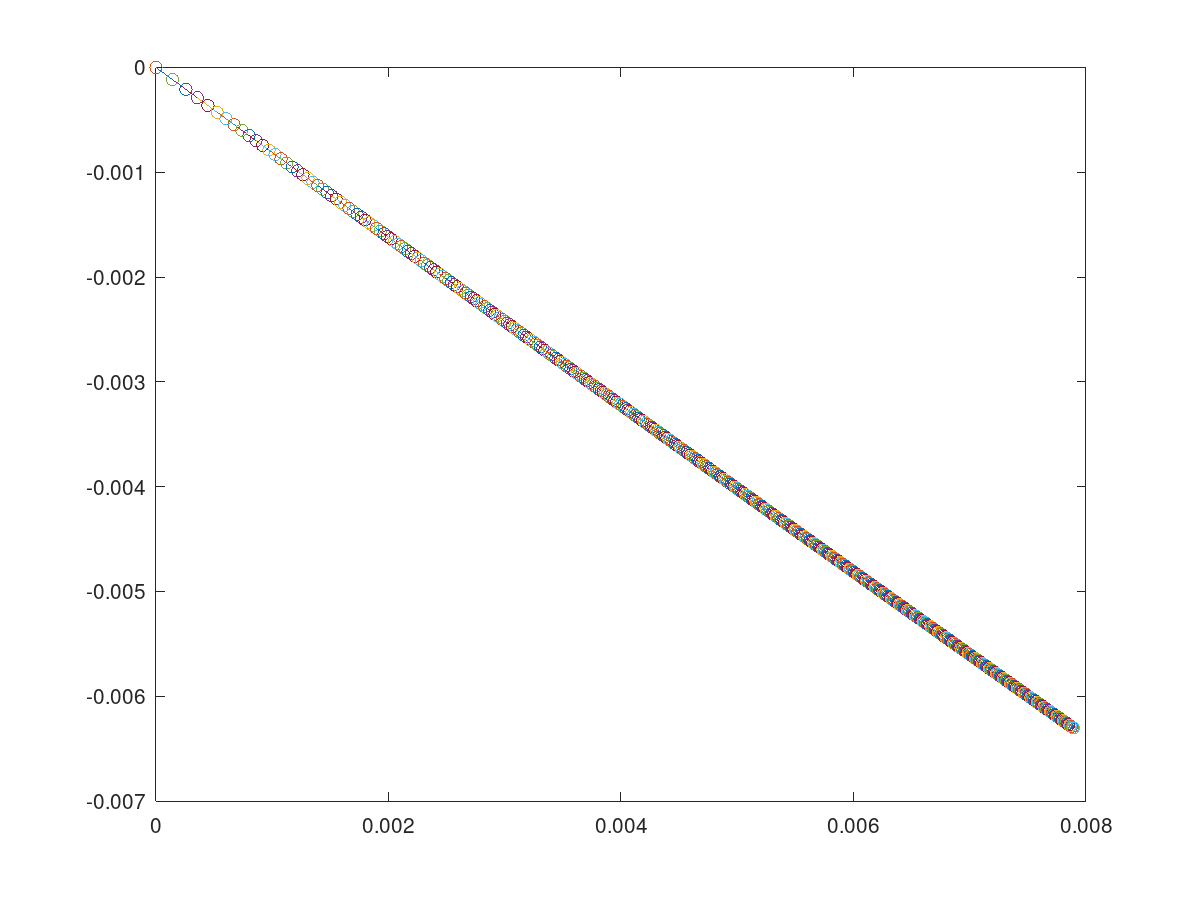
\includegraphics[width=7.5cm]{sgd_over_step_0_001}
        \caption{Progression of W using step of 0.001}
        \label{fig:sgd-over-0_001}
    \end{subfigure}
    \hfill
    % caption and label
    \caption{Progression of W for overdetermined system using SGD}
    \label{fig:sdg-over}
\end{figure}

\newpage

%========================
\subsection{Adam}
%========================

%------------------------
\subsubsection{Underdetermined}
%------------------------

% code
\lstinputlisting[language=Octave]{../Q1/adam_under.m}

% insert plots
\begin{figure}[H]
    \centering
    % digit 0
    \begin{subfigure}{0.48\textwidth}
        \centering
        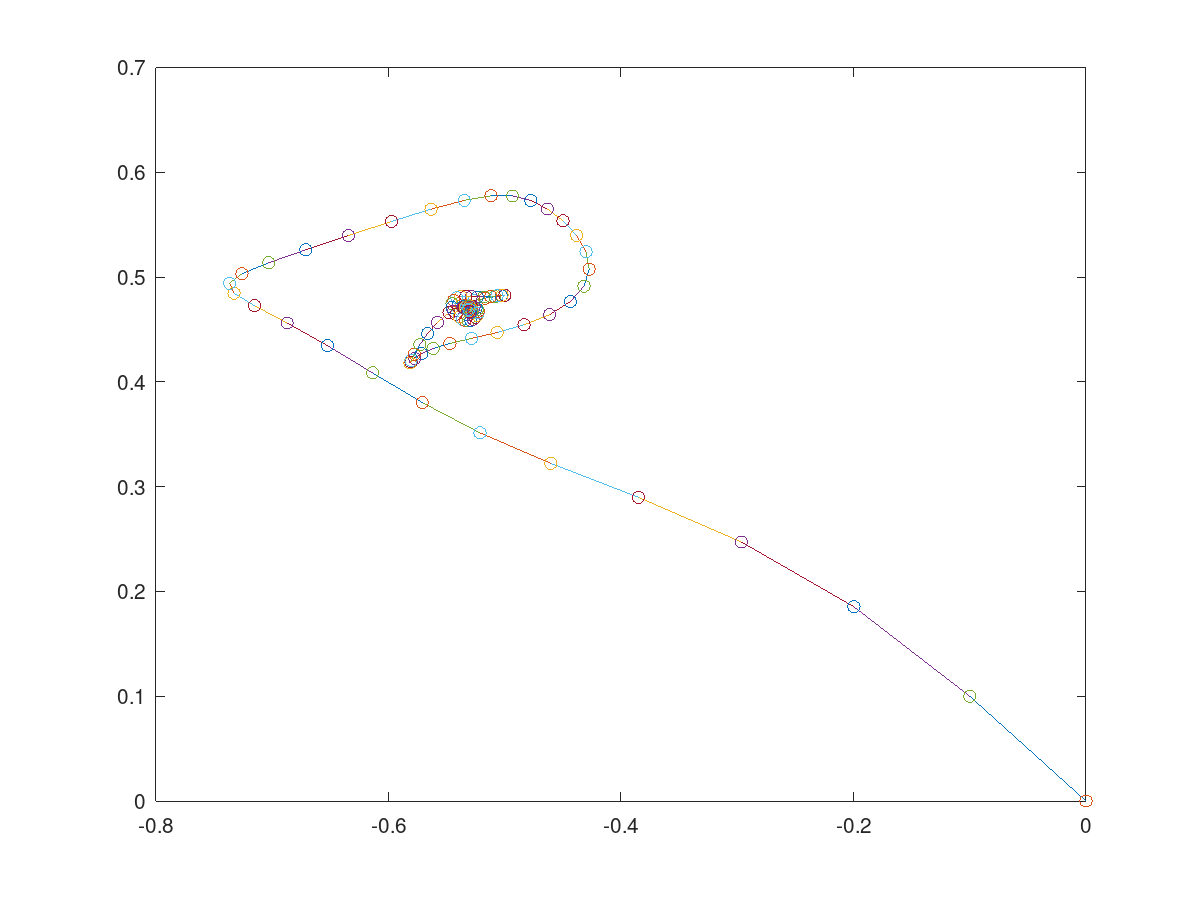
\includegraphics[width=7.5cm]{adam_under_step_0_1}
        \caption{Progression of W using step of 0.1}
        \label{fig:adam-under-0_1}
    \end{subfigure}
    \hfill
    % digit 1
    \begin{subfigure}{0.48\textwidth}
        \centering
        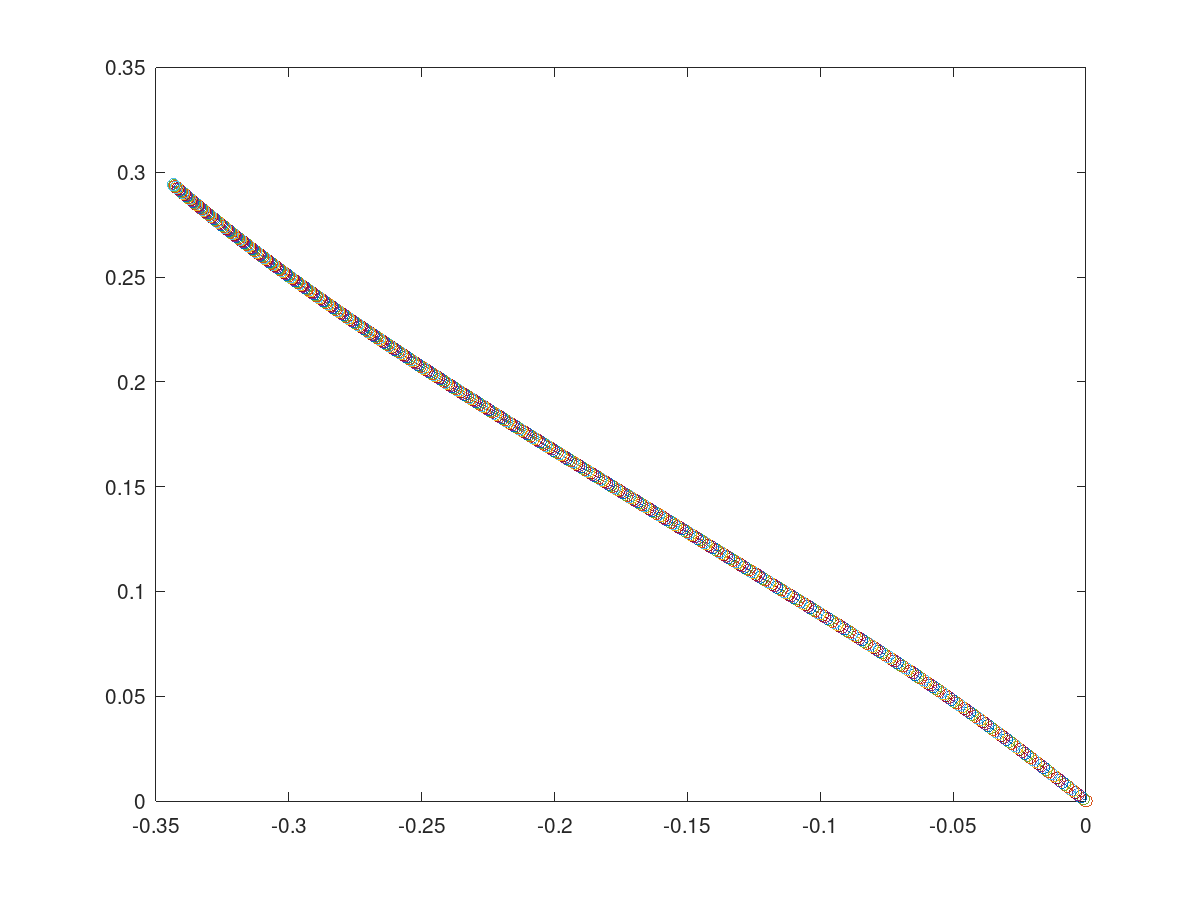
\includegraphics[width=7.5cm]{adam_under_step_0_001}
        \caption{Progression of W using step of 0.001}
        \label{fig:adam-under-0_001}
    \end{subfigure}
    \hfill
    % caption and label
    \caption{Progression of W for underdetermined system using Adam}
    \label{fig:adam-under}
\end{figure}

\newpage

%------------------------
\subsubsection{Overdetermined}
%------------------------

% code
\lstinputlisting[language=Octave]{../Q1/adam_over.m}

% insert plots
\begin{figure}[H]
    \centering
    % digit 0
    \begin{subfigure}{0.48\textwidth}
        \centering
        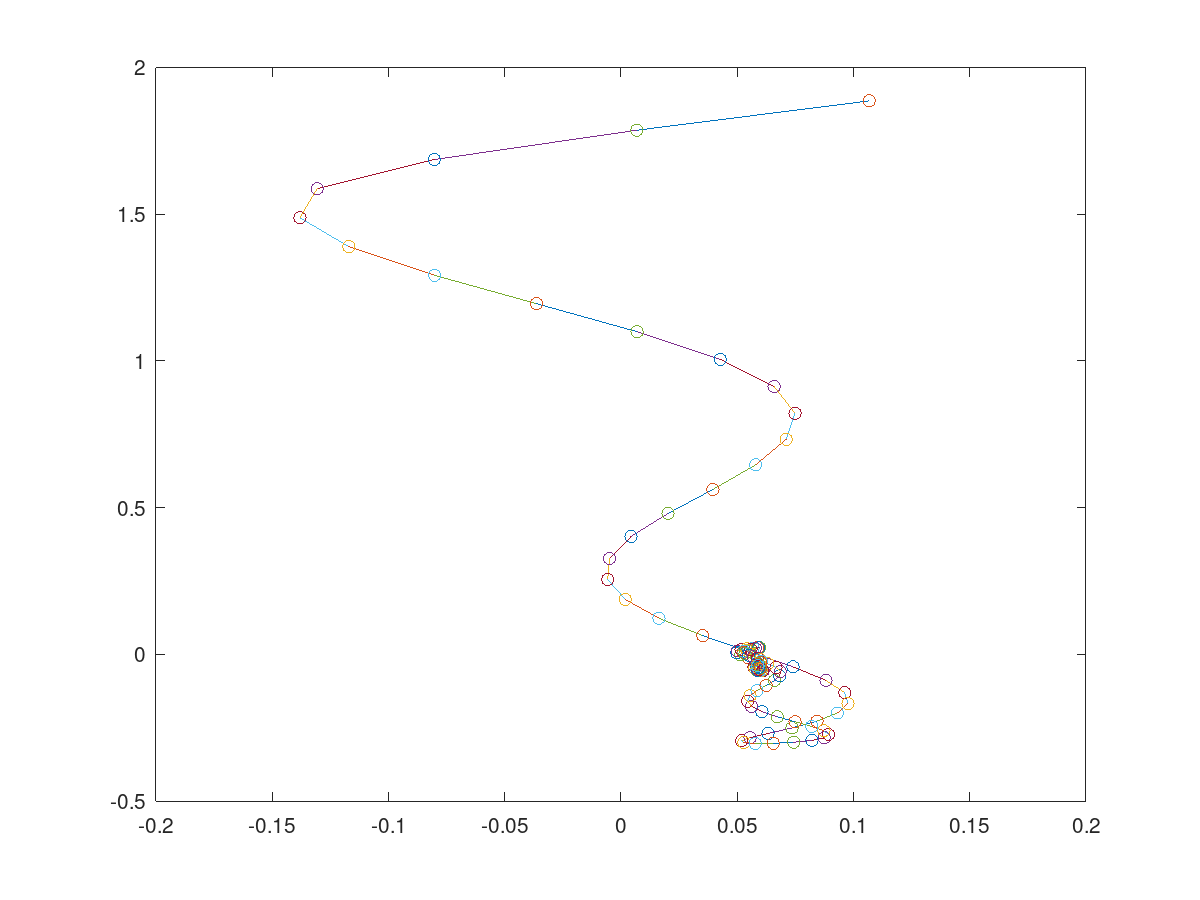
\includegraphics[width=7.5cm]{adam_over_step_0_1}
        \caption{Progression of W using step of 0.1}
        \label{fig:adam-over-0_1}
    \end{subfigure}
    \hfill
    % digit 1
    \begin{subfigure}{0.48\textwidth}
        \centering
        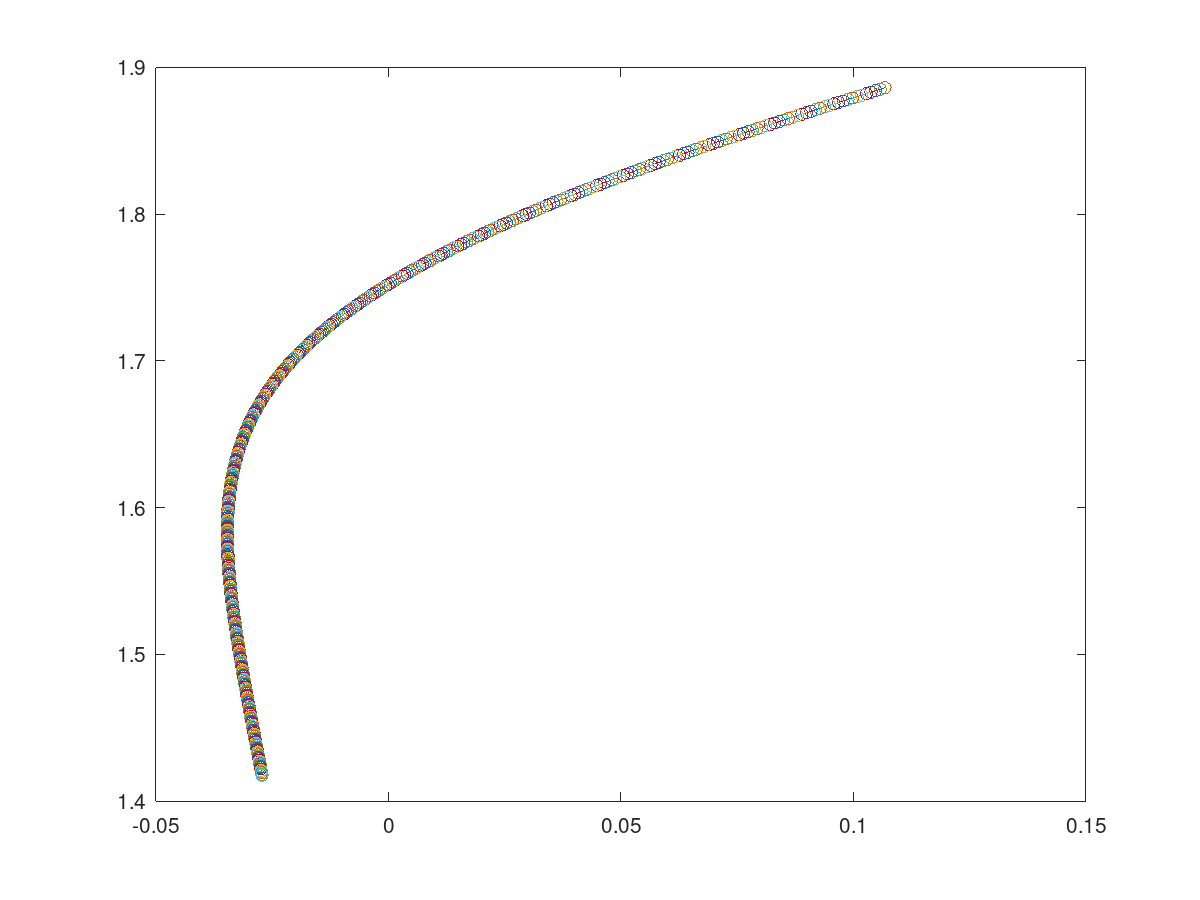
\includegraphics[width=7.5cm]{adam_over_step_0_001}
        \caption{Progression of W using step of 0.001}
        \label{fig:adam-over-0_001}
    \end{subfigure}
    \hfill
    % caption and label
    \caption{Progression of W for overdetermined system using Adam}
    \label{fig:adam-over}
\end{figure}

\newpage

%========================
\subsection{Comparison}
%========================

\paragraph{We can see from the plots that for SGD both underdetermined and overdetermined systems converged to the right solution using step equal to 0.1. When using step equal to 0.001, the optimizer did not converged, but we can see that it is on the way, not reaching it possibly because of the step value.}

\paragraph{The same thing happened when using Adam optimizer. For steps equal to 0.1, both underdetermined and overdetermined converged to the right solution}

\paragraph{Comparing both plots, in general we can see that SGD has a smoother path, walking directly to the solution. Adam, on the other hand, due to the adaptative moment estimation, shows a curlier path through the solution.}

\newpage

%=================================================
\section*{Question 2}
%=================================================

\[min\|Ax-b\|_{P}^{2}+\|x-x_{0}\|_{Q}^{2}\]
%------------------------
\paragraph{Since we are searching for $x$ that minimizes the previous expression, we will calculate the derivative with relation to $x$ and set it equal to zero:}
    \[\frac{d}{dx} (\|Ax-b\|_{P}^{2}+\|x-x_{0}\|_{Q}^{2}) = 0\]
%------------------------
\paragraph{Property used: $\|x\|_{Q}^{2} = x^{T}Qx$}
    \[\frac{d}{dx} [\overbrace{(Ax-b)^{T} P (Ax-b)}^{\|Ax-b\|_{P}^{2}} + \overbrace{(x-x_0)^T Q (x-x_0)}^{\|x-x_{0}\|_{Q}^{2}}] = 0\]
%------------------------
\paragraph{Property used: $(M + N)^T = M^T + N^T$}
    \[\frac{d}{dx} \{[(Ax)^T-b^T] P (Ax-b) + (x^T-x_0^T) Q (x-x_0)\} = 0\]
%------------------------
\paragraph{Property used: $(MN)^T = N^T M^T$}
    \[\frac{d}{dx} \{[x^TA^T-b^T] P (Ax-b) + (x^T-x_0^T) Q (x-x_0)\} = 0\]
    \[\frac{d}{dx} [(x^TA^TPAx - x^TA^TPb -b^TPAx + b^TPb) + (x^TQx - x^TQx_0 - x_0^TQx + x_0^TQx_0)] = 0\]
%------------------------
\paragraph{Properties used:}
    \begin{itemize}
        \item $\frac{d}{dy}(y^TMy) = M^Ty + My$.
        \item $\frac{d}{dy}(y^TMy) = 2My$, if $M = M^T$ (i.e. $M$ is symmetric)
        \item $\frac{d(Ax)}{dx} = A$
        \item $\frac{d(x^TA)}{dx} = A^T$
        \item obs.: $A^TPA$ is symmetric, since $(A^TPA)^T = (PA)^T(A^T)^T = A^TP^TA$, but $P^T = P$, since P is symmetric. Then $A^TPA = (A^TPA)^T$
    \end{itemize}
\paragraph{Using the previous properties, we have:}
    \[\frac{d}{dx} [(x^TA^TPAx - x^TA^TPb -b^TPAx + b^TPb) + (x^TQx - x^TQx_0 - x_0^TQx + x_0^TQx_0)] = 0\]
    \[[2A^TPAx - (A^TPb)^T - b^TPA + 0] + [2Qx - (Qx_0)^T - x_0^TQ + 0] = 0\]
    \[2A^TPAx - (Pb)^T(A^T)^T - b^TPA + 2Qx - x_0^TQ^T - x_0^TQ = 0\]
    \[2A^TPAx - b^TP^TA - b^TPA + 2Qx - x_0^TQ - x_0^TQ = 0\]
    \[2A^TPAx - b^TPA - b^TPA + 2Qx - x_0^TQ - x_0^TQ = 0\]
    \[2A^TPAx - 2b^TPA + 2Qx - 2x_0^TQ = 0\]
    \[2A^TPAx + 2Qx = 2b^TPA + 2x_0^TQ\]
    \[A^TPAx + Qx = b^TPA + x_0^TQ\]
    \[(A^TPA + Q)^{-1}(A^TPA + Q)x = (A^TPA + Q)^{-1}(b^TPA + x_0^TQ)\]
    \[x = (A^TPA + Q)^{-1}(b^TPA + x_0^TQ)\]
    \[x = (A^TPA + Q)^{-1}(b^TP^TA + x_0^TQ^T)\]
    \[x = (A^TPA + Q)^{-1}[(Pb)^TA + (Qx_0)^T]\]
    \[x = (A^TPA + Q)^{-1}[(A^TPb)^T + (Qx_0)^T]\]
    \[\boxed{x = (A^TPA + Q)^{-1}(A^TPb + Qx_0)^T}\]
%------------------------
%\paragraph{Properties used:}
%    \begin{itemize}
%        \item Since $Q$ is symmetric, $(Qx_0)^T = Qx_0$
%        \item Since $P$ is symmetric, $(A^TPb)^T = (A^TPb)$
%    \end{itemize}
%\paragraph{Then:}
%    \[x = (A^TPA + Q)^{-1}[(A^TPb)^T + (Qx_0)^T]\]
%    \[x = (A^TPA + Q)^{-1}(A^TPb + Qx_0)\]
%------------------------

\paragraph{If the regularization coefficient was used, we would have:}
    \[min\|Ax-b\|_{P}^{2}+\alpha^2\|x-x_{0}\|_{Q}^{2}\]

\paragraph{This, would lead to the solution:}
\[x = (A^TPA + \alpha^2Q)^{-1}(A^TPb + \alpha^2Qx_0)^T\]

\paragraph{So, even if we choose an $\alpha$ different than 1, it is always possible to embed its value in the matrix $Q$, since $\alpha$ is only multiplying the $Q$ matrix.}

\newpage

%=================================================
\section*{Question 3}
%=================================================

%------------------------
\subsection*{a)}
%------------------------

\paragraph{If $M$ is symmetric, then $M^T$ must be equal to $M$:}
    \[M^T = (N^TN)^T = N^T(N^T)^T = N^TN = M\]
\paragraph{Now we need to prove that $M$ must be positive semi-definite, i.e., $z^TMz \geq 0, \forall z \in R^n$:}
    \[z^TMz = z^T(N^TN)z = (z^TN^T)(Nz) = (Nz)^T(Nz) = \|Nz\|^2 \geq 0\]

%------------------------
\subsection*{b)}
%------------------------

\paragraph{...}


%------------------------
\subsection*{c)}
%------------------------

\paragraph{We want to prove that $N$ may not be unique in $M=N^TN$. For this, lets consider the orthogonal matrix $Q$ and the new matrix that is the result by its multiplication with $N$, i.e., $QN$:}
    \[M = (QN)^T(QN) = (N^TQ^T)(QN) = N^T(Q^TQ)N\]

\paragraph{Since $Q$ is orthogonal, $Q^TQ$ is equal to the identity matrix $I$. Hence:}
    \[M= N^T(Q^TQ)N = N^TIN = N^TN\]

\paragraph{So if $M$ can be decomposed in $N^TN$, it can also be decomposed by $(QN)^T(QN)$, with $Q$ being an orthogonal matrix.}

%------------------------
\subsection*{d)}
%------------------------

\paragraph{In order to find $N$ we can use Cholesky decomposition. Here we will show an example for n = 3, but we will generalize to other dimensions:}

\begin{align*}
    M = N^TN & =
    \begin{pmatrix}   N_{11} & 0 & 0 \\
        N_{21} & N_{22} & 0 \\
        N_{31} & N_{32} & N_{33}\\
    \end{pmatrix}
    \begin{pmatrix}   N_{11} & N_{21} & N_{31} \\
        0 & N_{22} & N_{32} \\
        0 & 0 & N_{33}
    \end{pmatrix} \\
    & =
    \begin{pmatrix}   N_{11}^2 &   &(\text{symmetric})   \\
        N_{21}N_{11} & N_{21}^2 + N_{22}^2& \\
        N_{31}N_{11} & N_{31}N_{21}+N_{32}N_{22} & N_{31}^2 + N_{32}^2+N_{33}^2
    \end{pmatrix}
\end{align*}

Comparing to the elements of $M$ we can find $N$:

\begin{align*}
    N = 
    \begin{pmatrix} \sqrt{M_{11}} &  0 & 0  \\
    M_{21}/N_{11} & \sqrt{M_{22} - N_{21}^2} & 0 \\
    M_{31}/N_{11} &  \left( M_{32} - N_{31}N_{21} \right) /N_{22}  &\sqrt{M_{33}- N_{31}^2 - N_{32}^2}
    \end{pmatrix}
\end{align*}

Generalizing for other dimensions, we have:
\[\boxed{N_{j,j} = (\pm)\sqrt{ M_{j,j} - \sum_{k=1}^{j-1} N_{j,k}^2 }}\]
\begin{center}for elements at the diagonal\end{center}

\[\boxed{N_{i,j} = \frac{1}{N_{j,j}} \left( M_{i,j} - \sum_{k=1}^{j-1} N_{i,k} N_{j,k} \right)}\]
\begin{center}for i$>$j\end{center}


\newpage

%=================================================
\section*{Question 4}
%=================================================

\paragraph{The Taylor series expansion of a function $f(x,y)$ in a neighborhood around $(x_0,y_0)$ is as follows:}
    \[f(x,y) \approx f(x_0,y_0) + \underbrace{f_x(x_0,y_0)(x-x_0)+f_y(x_0,y_0)(y-y_0)}_{\text{first order term}} + ...\]

\paragraph{Ignoring terms from second order and higher, and considering the linearized function given $f_L(x,y)=2x+py-8$, we have:}
    \[f_L(x,y) = f(x_0,y_0) + f_x(x_0,y_0)(x-x_0)+f_y(x_0,y_0)(y-y_0)\]

\paragraph{Taking $f(x,y) = x\sqrt y$, we have:}
\begin{itemize}
    \item $f_x(x,y) = \sqrt y$
    \item $f_y(x,y) = \frac{x}{2\sqrt y}$
\end{itemize}
    \[2x+py-8 = \underbrace{x_0\sqrt y_0}_{f(x_0,y_0)} + \underbrace{\sqrt y_0}_{f_x(x_0,y_0)}(x-x_0) + \underbrace{\frac{x_0}{2\sqrt y_0}}_{f_y(x_0,y_0)}(y-y_0)\]
    \[2x+py-8 = x_0\sqrt y_0 + x\sqrt y_0 - x_0\sqrt y_0 + \frac{x_0 y}{2\sqrt y_0} - \frac{x_0 y_0}{2\sqrt y_0}\]
    \[2x+py-8 =  \sqrt y_0 x + \left(\frac{x_0}{2\sqrt y_0}\right) y - \left(\frac{x_0 y_0}{2\sqrt y_0}\right)\]
    
    \paragraph{Now, if we compare the terms that only depend on $x$, that only depend on $y$ and the independent terms (that only depend on $x_0$ and $y_0$), we have:}
\begin{itemize}
    \item (i)   $ 2 = \sqrt y_0 \implies \boxed{y_0 = 4}$ 
    \item (ii)  $ p = \left(\frac{x_0}{2\sqrt y_0}\right) $
    \item (iii) $ 8 = \left(\frac{x_0 y_0}{2\sqrt y_0}\right) $
\end{itemize}

\paragraph{Substituting in (i) in (iii):}
    \[\frac{x_0 y_0}{2\sqrt y_0} = 8\]
    \[\frac{4 x_0}{2\cdot2} = 8\]
    \[\boxed{x_0 = 8}\]

\paragraph{Substituting in (ii):}
    \[p = \frac{x_0}{2\sqrt y_0}\]
    \[p = \frac{8}{2\cdot2}\]
    \[\boxed{p = 2}\]

    \paragraph{So the point from where the function was linearized is $(x_0,y_0) = (8,4)$ and the coefficient $p = 2$, then $f_L(x,y) = 2x + 2y -8$.}

\newpage
 
%=================================================
\section*{Question 5}
%=================================================
\addtocounter{section}{1}

%==================================
\subsection*{\underline{Dedução:}}
%==================================

%------------------------
\subsubsection*{\hspace{5mm}$\bullet$ Explicação:}
%------------------------
\paragraph{Na inferência dedutiva a conclusão sempre está contida nas premissas. Ao derivar uma afirmação $y$ partindo de $x$, dizemos que $y$ é uma consequência lógica de $x$, ou seja, a inferência de $y$ é baseada no que foi assumido em $x$ e será sempre verdadeira. Também podemos incluir casos particulares que são inferidos a partir de premissas universais e gerais.}

%------------------------
\subsubsection*{\hspace{5mm}$\bullet$ Vantagem:}
%------------------------
\paragraph{Dos três tipos de inferência esta é a única cuja conclusão lógica é sempre verdadeira.}

%------------------------
\subsubsection*{\hspace{5mm}$\bullet$ Desvantagem:}
%------------------------
\paragraph{É a única das inferências que não acrescenta conhecimento novo.}

%------------------------
\subsubsection*{\hspace{5mm}$\bullet$ Exemplo:}
%------------------------
\paragraph{Se um pesquisador estiver treinando uma rede neural e por algum motivo as informações referentes ao estado atual do treinamento seja perdido (seja por falta de energia, Colab retomando a máquina virtual, ou qualquer outro) sem que haja um backup dos pesos e parâmetros, será necessário reiniciar o treinamento do zero. Logo, o pesquisador opta por salvar checkpoints do status do treinamento (pesos e outros parâmetros), para caso isso ocorra, o treinamento não seja inteiramente perdido e o pesquisador possa continuar do último estado salvo. Essa ação preventiva é tomada baseada em uma inferência dedutiva.\\
1. Se cai a energia e não tenho backup $\implies$ perco o treinamento\\
2. Quando perco o treinamento (sem backup) $\implies$ recomeço do zero\\
%
conclusão: se cai energia sem backup, perco tempo recomeçando do zero.\\
precaução: vou salvar checkpoints do treinamento.}

%==================================
\subsection*{\underline{Indução:}}
%==================================

%------------------------
\subsubsection*{\hspace{5mm}$\bullet$ Explicação:}
%------------------------
\paragraph{Diferente da dedução aqui não temos mais a garantia de veracidade a cerca de inferência. Em indução temos a intuição de probabilidade, agregando experiência e conhecimento. A partir de um certo conjunto de elementos conhecidos ou observáveis, e portanto de casos particulares, chega-se em uma conclusão geral. Assim, uma característica marcante deste tipo de inferência é a capacidade de generalização.}

%------------------------
\subsubsection*{\hspace{5mm}$\bullet$ Vantagem:}
%-----------------------
\paragraph{Entre as vantagens deste modo de inferência podemos listar a capacidade de generalização mesmo sem haver uma certeza lógica e uso de experiências anteriores a cerca do que se está inferindo.}

%------------------------
\subsubsection*{\hspace{5mm}$\bullet$ Desvantagem:}
%------------------------
\paragraph{Esta inferência não é 100\% verdade como a dedutiva, portanto pode levar a generalizações errôneas. Por trabalhar com experiências passadas, tem potencial de acrescentar informação menor do que a abdução, pois boa parte dela foi usada como experiência para a própria inferência.}

%------------------------
\subsubsection*{\hspace{5mm}$\bullet$ Exemplo:}
%------------------------
\paragraph{Ao rodar o loop de treinamento de uma rede neural, o pesquisador se depara com uma exceção Python por conta de um erro em operações envolvendo matrizes que apresenta um log de erro não direto e difícil de interpretar, não sendo muito útil portanto. Em experiências anteriores, na maior parte das vezes o erro era causado por descasamento nos shapes de tensores/arrays ou dimensões erradas. Assim, o pesquisador decide usar um debugger (ex: pdb) colocando o breakpoint imediatamente na linha antes do erro acontecer e checar os shapes e dimensões dos tensores envolvidos, pois desconfia que o erro envolva uma dessas duas coisas.}

%==================================
\subsection*{\underline{Abdução:}}
%==================================

%------------------------
\subsubsection*{\hspace{5mm}$\bullet$ Explicação:}
%------------------------
\paragraph{Na inferência abdutiva trabalha-se com hipóteses para explicação do que foi observado. Trata-se de inferir $x$ como explicação para $y$. A conclusão não é dado pela lógica, mas sim pela capacidade em justificar e argumentar a escolha da melhor hipótese dado um contexto. Mesmo que este tipo de inferência não tenha a certeza da inferência dedutiva, cria-se conclusões que nos fazem considerar a hipótese como plausível e/ou verdadeira.}

%------------------------
\subsubsection*{\hspace{5mm}$\bullet$ Vantagem:}
%------------------------
\paragraph{Dos três tipos de inferência esta é a que mais pode acrescentar informação, caso a inferência seja condizente com a realidade e possa se sustentar com argumentos. Quando usada adequadamente, pode ser bastante útil informações a priori (priors) em estatística Bayesiana.}

%------------------------
\subsubsection*{\hspace{5mm}$\bullet$ Desvantagem:}
%------------------------
\paragraph{Entretanto, é mais fraca do ponto de vista lógico, no sentido de não haver certeza alguma no que se está concluindo, havendo apenas formação de hipóteses que podem sustentar a análise.}

%------------------------
\subsubsection*{\hspace{5mm}$\bullet$ Exemplo:}
%------------------------
\paragraph{O pesquisador está pela primeira vez trabalhando big data que requer uso intenso de GPU, horas de processamento, milhões de amostras, milhões de parâmetros ajustáveis, etc. Ele está treinando uma arquitetura do T5 da Google para traduzir sentenças do inglês para português. Ao iniciar o treinamento percebe que o tempo de processamento de uma época está na ordem de 10 horas. Como o pesquisador não dispõe de tempo para treinar por algumas épocas, decide que precisa diminuir o tempo de treinamento, mas tentando perder o mínimo de qualidade possível. Assim, o pesquisador decide tentar usar uma precisão de 16-bits ao invés da tradicional 32-bits. Essa foi uma escolha dentre inúmeras outras (abaixar batch size, aumentar learning rate, dimunuir tamanho das sequências de entrada/saída, usar um modelo menos parâmetros, alterar o scheduling factor, etc). Dentre todas as ações a se tomar, o pesquisador toma como primeiro palpite a tentativa de usar outro valor de precisão, com o pensamento de que este pode oferecer o melhor tradeoff entre custo computacional, mantendo qualidade na tradução de seu modelo.}

%==================================
\subsection*{Por quê treinar uma rede neural está associado a um processo de inferência indutiva?}
%==================================

\paragraph{No treinamento de uma rede neural, um dos principais conceitos está no aprendizado através de dados. O que procura-se no treinamento, é a distrubuição original e desconhecida que gerou os dados, para que se possa generalizar para além dos dados que se dispõe. Assim, se pudermos modelar uma distribuição, baseado nos dados de treinamento, podemos tirar conclusões a respeito de qualquer dado possível que esteja submetido àquela distribuição (se a generalização estiver boa).\\
Uma das definições de aprendizado de máquina, dada por Tom Mitchell (1997) é: "diz-se que um programa de computador aprendeu de uma experiência E com respeito a uma certa tarefa T e com certa performance P, se sua performance em T medida por P aumenta com a experiência E". Nessa afirmação, pode-ser ver claramente os príncipios de inferência indutiva, havendo a questão da experiência em E e capacidade de generalização em T medida por P.\\
Por fim, temos exatamente a situação em que parte-se de casos particulares (dados de treinamento) a fim de se inferir o caso geral (distruição que gerou os dados / capacidade de generalização).}

\newpage

%=================================================
\section*{Question 6}
%=================================================

\paragraph{O primeiro paper selecionado é de 2002 com 2173 citações. Esse paper foi publicado no JAMA (The Journal of the American Medical Association) que é um jornal da área médica com 48 publicações por ano pela AMA (American Medical Association).}
\begin{itemize}
    \item \textbf{title:} Effects of Cognitive Training Interventions With Older Adults - A Randomized Controlled Trial
    \item \textbf{year:} 2002
    \item \textbf{cited by:} 2173
    \item \textbf{publication:} JAMA
    \item \textbf{reference:} Ball K, Berch DB, Helmers KF, et al. Effects of Cognitive Training Interventions With Older Adults: A Randomized Controlled Trial. JAMA. 2002;288(18):2271–2281.\\ doi:10.1001/jama.288.18.2271
\end{itemize}

%------------------------

\paragraph{O segundo paper selecionado é de 2009 e conta com 315 citações. Esse paper foi publicado no jornal acadêmico Alzheimer's \& Dementia, que conta com publicações mensais da associação sem fins lucrativos Journal of the Alzheimer's Association.}

\begin{itemize}
    \item \textbf{title:} Immediate and delayed effects of cognitive interventions in healthy elderly: A review of current literature and future directions
    \item \textbf{year:} 2009
    \item \textbf{cited by:} 315
    \item \textbf{publication:} Alzheimer's \& Dementia (Volume 5, Issue 1, January 2009, Pages 50-60)
    \item \textbf{reference:} Papp K V, Walsh S J, Snyder P J. Immediate and delayed effects of cognitive interventions in healthy elderly: a review of current literature and future directions. Alzheimer's and Dementia 2009; 5(1): 50-60. [PubMed]
\end{itemize}

%=================================================

\end{document}
